\documentclass{beamer}

\usepackage{graphics}
\usetheme{metropolis}           % Use metropolis theme
\usepackage{color}
\usepackage{amssymb}
\usepackage{amsmath}
\usepackage{mathtools}
\usepackage{amstext}
\usepackage{blindtext}
\usepackage{float}
\usepackage{csquotes}
\usepackage{todonotes}
\usepackage{afterpage}
\usepackage{caption}
\usepackage{framed}

\usepackage{hyperref}
\usepackage{cite}
%\usepackage{listings}
\usepackage{booktabs} % Required for better horizontal rules in tables
\usepackage{multirow}
\usepackage{multicol}
\usepackage{graphicx}

%\usepackage[
%backend=bibtex,
%style=nature   ,
%]{biblatex}

%\addbibresource{library.bib}


\title{Planning and Scheduling at home project}
\date{\today}
\author{\'{A}ngela Patricia Enr\'{i}quez G\'{o}mez, Ethan Oswald Massey, Maximilian Mensing}
\institute{BRSU}
\begin{document}
\maketitle


\section{Introduction}

\begin{frame}{\textsl{ Task }}

  Storing Groceries

  \begin{itemize}
    \item \textbf{Case 1}: Everything is known. One object is on the table and has to be placed at any shelf after the cupboard has been opened.
    \item \textbf{Case 2}: The amount of Objects, the table and the cupboard have to be located. The objects have to be placed on the shelves.
    \item \textbf{Case 3}: As case 2 - In addition to not knowing the number of objects, the objects themself are also unknown.
    \item \textbf{Case 4}: In addition to case 3 the cupboard is unknown and has to be explored. The items have to be put in different categories and sorted by category on the shelf.
  \end{itemize}

\end{frame}

\begin{frame}{\textsl{Selection of the Planner}}

  \begin{figure}
    \centering
    \includegraphics[width=0.99\linewidth]{jshop_comparision}
    \label{fig:kim}
  \end{figure}

\end{frame}


\begin{frame}{\textsl{Using JSHOP2}}
  \begin{itemize}
    \item Get jshop from \url{https://github.com/mas-group/jshop2}
    \item Set environment \textbf{{\tiny export CLASSPATH="`pwd`/bin.build/JSHOP2.jar:`pwd`/antlr.jar:."}}
    \item Compile using \textbf{{\tiny make c}}
    \item Run by calling \textbf{{\tiny make problem1/2/3/4}}
  \end{itemize}

\end{frame}




\begin{frame}{Domain Overview}
  \begin{itemize}
    \item Domain models include:
      \begin{itemize}
        \item operators
        \item methods
        \item axioms
      \end{itemize}
  \end{itemize}
\end{frame}

\begin{frame}{Domain Assumptions and Approach}
\item Common sense assumptions were made to limit domain complexity.
\item Assumptions include, but are not limited to:
  \begin{itemize}
    \item Position of all objects are known and static (unless acted on by the robot)
    \item There is exactly the number of objects required (e.g. only one table)
    \item The robot is able to sense and identify all objects correctly
  \end{itemize}

\item Testing began with the smallest domain (Problem 1) and gradually increase in complexity
\end{frame}


\section{Example - Problem 1}
\begin{frame}{What's in a Problem File}
  \begin{itemize}
    \item Problem files are created for each problem
    \item Contain inital state and the compond task to be solved
    \item HTN planner uses this to create a solution
  \end{itemize}
\end{frame}

\begin{frame}{Problem Outline}
  \begin{itemize}
    \item Location of the table and cupboard are known
    \item There is only one object on the table and it's location is known
    \item The cupboard door is closed
    \item The object can be placed on any shelf
  \end{itemize}
\end{frame}


\begin{frame}{Problem Definition}
  \begin{lstlisting}
  (defproblem problem1 storegroceries
    ;;Problem 1
    (
      (object a1)
      (cupboard c1)
      (door d1)
      (shelf s1)
      (table t1)
      (robot r1)
      (on a1 t1) (door-closed d1)(robot-at r1 t1)
    )
    ((move-known-object a1 t1 c1 s1))
  )
  \end{lstlisting}
\end{frame}


%\begin{frame}{Obtaining Results}
%  \begin{itemize}
%    \item Planning can by obtained simply by running: \verb|make problem1| \\
%    \item This results in the following plan with 6 primitve tasks:
%  \end{itemize}
%
%  \begin{lstlisting}
%  [ 1 ]    (!move r1 t1 c1)
%  [ 2 ]    (!open-door d1)
%  [ 3 ]    (!move r1 c1 t1)
%  [ 4 ]    (!pickup a1 t1)
%  [ 5 ]    (!move r1 t1 c1)
%  [ 6 ]    (!putdown a1 s1)
%  \end{lstlisting}
%\end{frame}

\begin{frame}{GUI Result}
  \begin{figure}[h!]
    \centering
    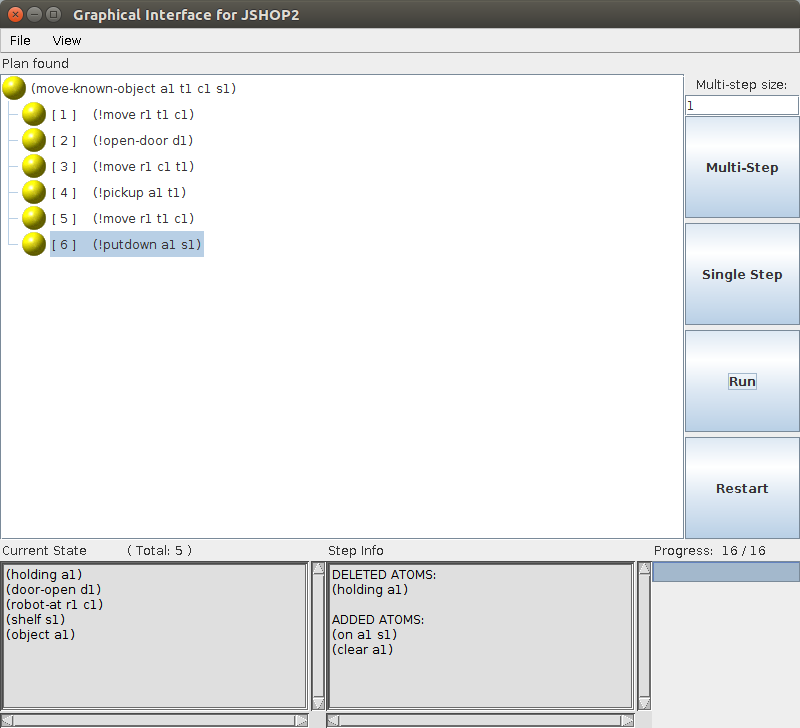
\includegraphics[width=0.65\linewidth]{images/problem1_gui}
    \caption{GUI Problem 1}
    \label{fig:probem1_gui}
  \end{figure}
\end{frame}


\section{Limitations and Issues}

\begin{frame}{Limitations}
  \begin{itemize}
    \item Without sufficient prior information the planner is not able to classify objects
    \item If assumptions are invalidated the planner will fail
    \item In problem 4, if the shelves don't have example objects  the planner has problems putting categories for them.
    \item Executing with java -ra generates all possible plans
      \begin{itemize}
        \item High space and time complexity
        \item Maximum of 4 objects to avoid outOfMemoryError
      \end{itemize}
  \end{itemize}
\end{frame}


\section{Diskussion}

\begin{frame}{Offene Punkte}
  \begin{itemize}

    \item
  \end{itemize}
\end{frame}


%%%%%%%%%%%%%%%%%%%  torcs -> parameter -> genom -> optimisation problem
%\printbibliography
%
\end{document}
